\documentclass[../main.tex]{subfiles}

\begin{document}

\subsection{Component Design}

\subsubsection{Meeple}

The meeple is the component that represents the player position on the board and gives feedback about player movement, death and turn role.

It consists on 2 LEDs, a green one and a yellow one, a hall sensor, a microcontroller (ESP-01) and a battery, as in the \textbf{Figure \ref{fig:meeple}}. Each component has the following function:

\begin{enumerate}
    \item \textbf{ESP-01}: Microcontroller that controls the LEDs, reads the Hall Sensor and reads/writes feedback with MQTT.
    \item \textbf{Battery}: Power source for the ESP-01
    \item \textbf{Hall Sensor}: Detects when the meeple is being detected on board, detects meeple movement and death.
    \item \textbf{Green LED}: Has two modes, when blinking it indicates that it's the meeple turn for moving, when solid it indicates the hall sensor is detecting a magnetic field (the meeple is detecting the board).
    \item \textbf{Yellow LED}: Indicates if the player has the bullet on the shooting stage.
\end{enumerate}

\begin{figure}[!htb]
    \centering
    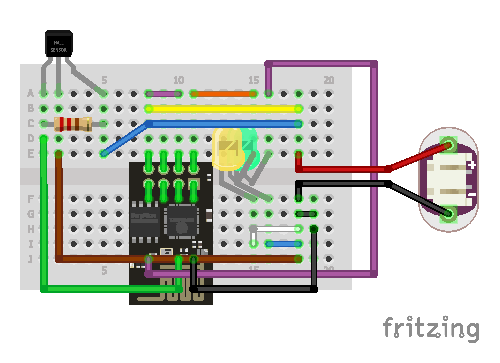
\includegraphics[width= 0.5\linewidth]{../media/figures/schematic_meeple.pdf}
    \caption{Meeple components schematic}
    \label{fig:meeple}
\end{figure}

\subsubsection{Operation base}

\subsubsection{Game Controller}



\subsubsection{Broker}

\end{document}